\chapter{Avaliação da plataforma}


\subsection{Uso do Noosfero na Disciplina de Manutenção e Evolução de Software}
\label{mes-unb}

Um exemplo do uso de uma rede de colaboração, como ambiente de apoio ao ensino,
pode ser visto no caso da disciplina do curso de Engenharia de Software de
Manutenção e Evolução de Software (MES), ministrada, no primeiro semestre de
2013, pelo professor Paulo Meirelles, na qual eu participei como monitor
voluntário.


A comunidade da disciplina de MES foi criada na rede da USP, com consentimento
da administração da mesma, pelo fato de que a rede Comunidade.UnB ainda estar
passando por uma fase de desenvolvimento e testes. Pretendemos apresentar
na segunda fase deste trabalho a ser apresentado no segundo semestre de 2013
uma pesquisa de satisfação dos alunos com o uso da plataforma na disciplina e
assim coletar \textit{feedbacks} e propostas de melhorias para a mesma. 

A disciplina teve como objetivo permitir com que os
alunos pudessem vivenciar situações reais de desenvolvimento de software ao
exercer atividades de manutenção, seja evolutiva, corretiva, perfectiva ou
qualquer outra forma de manutenção, em projetos de software livre e fez uso de
uma comunidade
~\footnote{Disponível em: \url{http://social.stoa.usp.br/mes-fga-unb/ementa}}
criada na rede de colaboração da USP, o Stoa, como ferramenta de comunicação a ser
utilizado pelo grupo e para a publicação dos resultados dos projetos.
%
A turma foi divida em grupos que selecionaram o projeto, dentro de uma lista
de opções fornecidas pelo professor, no qual desejavam atuar. Foi criado um 
sub-grupo, que funciona como uma comunidade normal, porém vinculada à comunidade
da disciplina, para cada projeto da disciplina. A Figura \ref{mes-unb}
apresenta a página da ementa da comunidade supracitada. 

\begin{figure}[h]
	\centering
	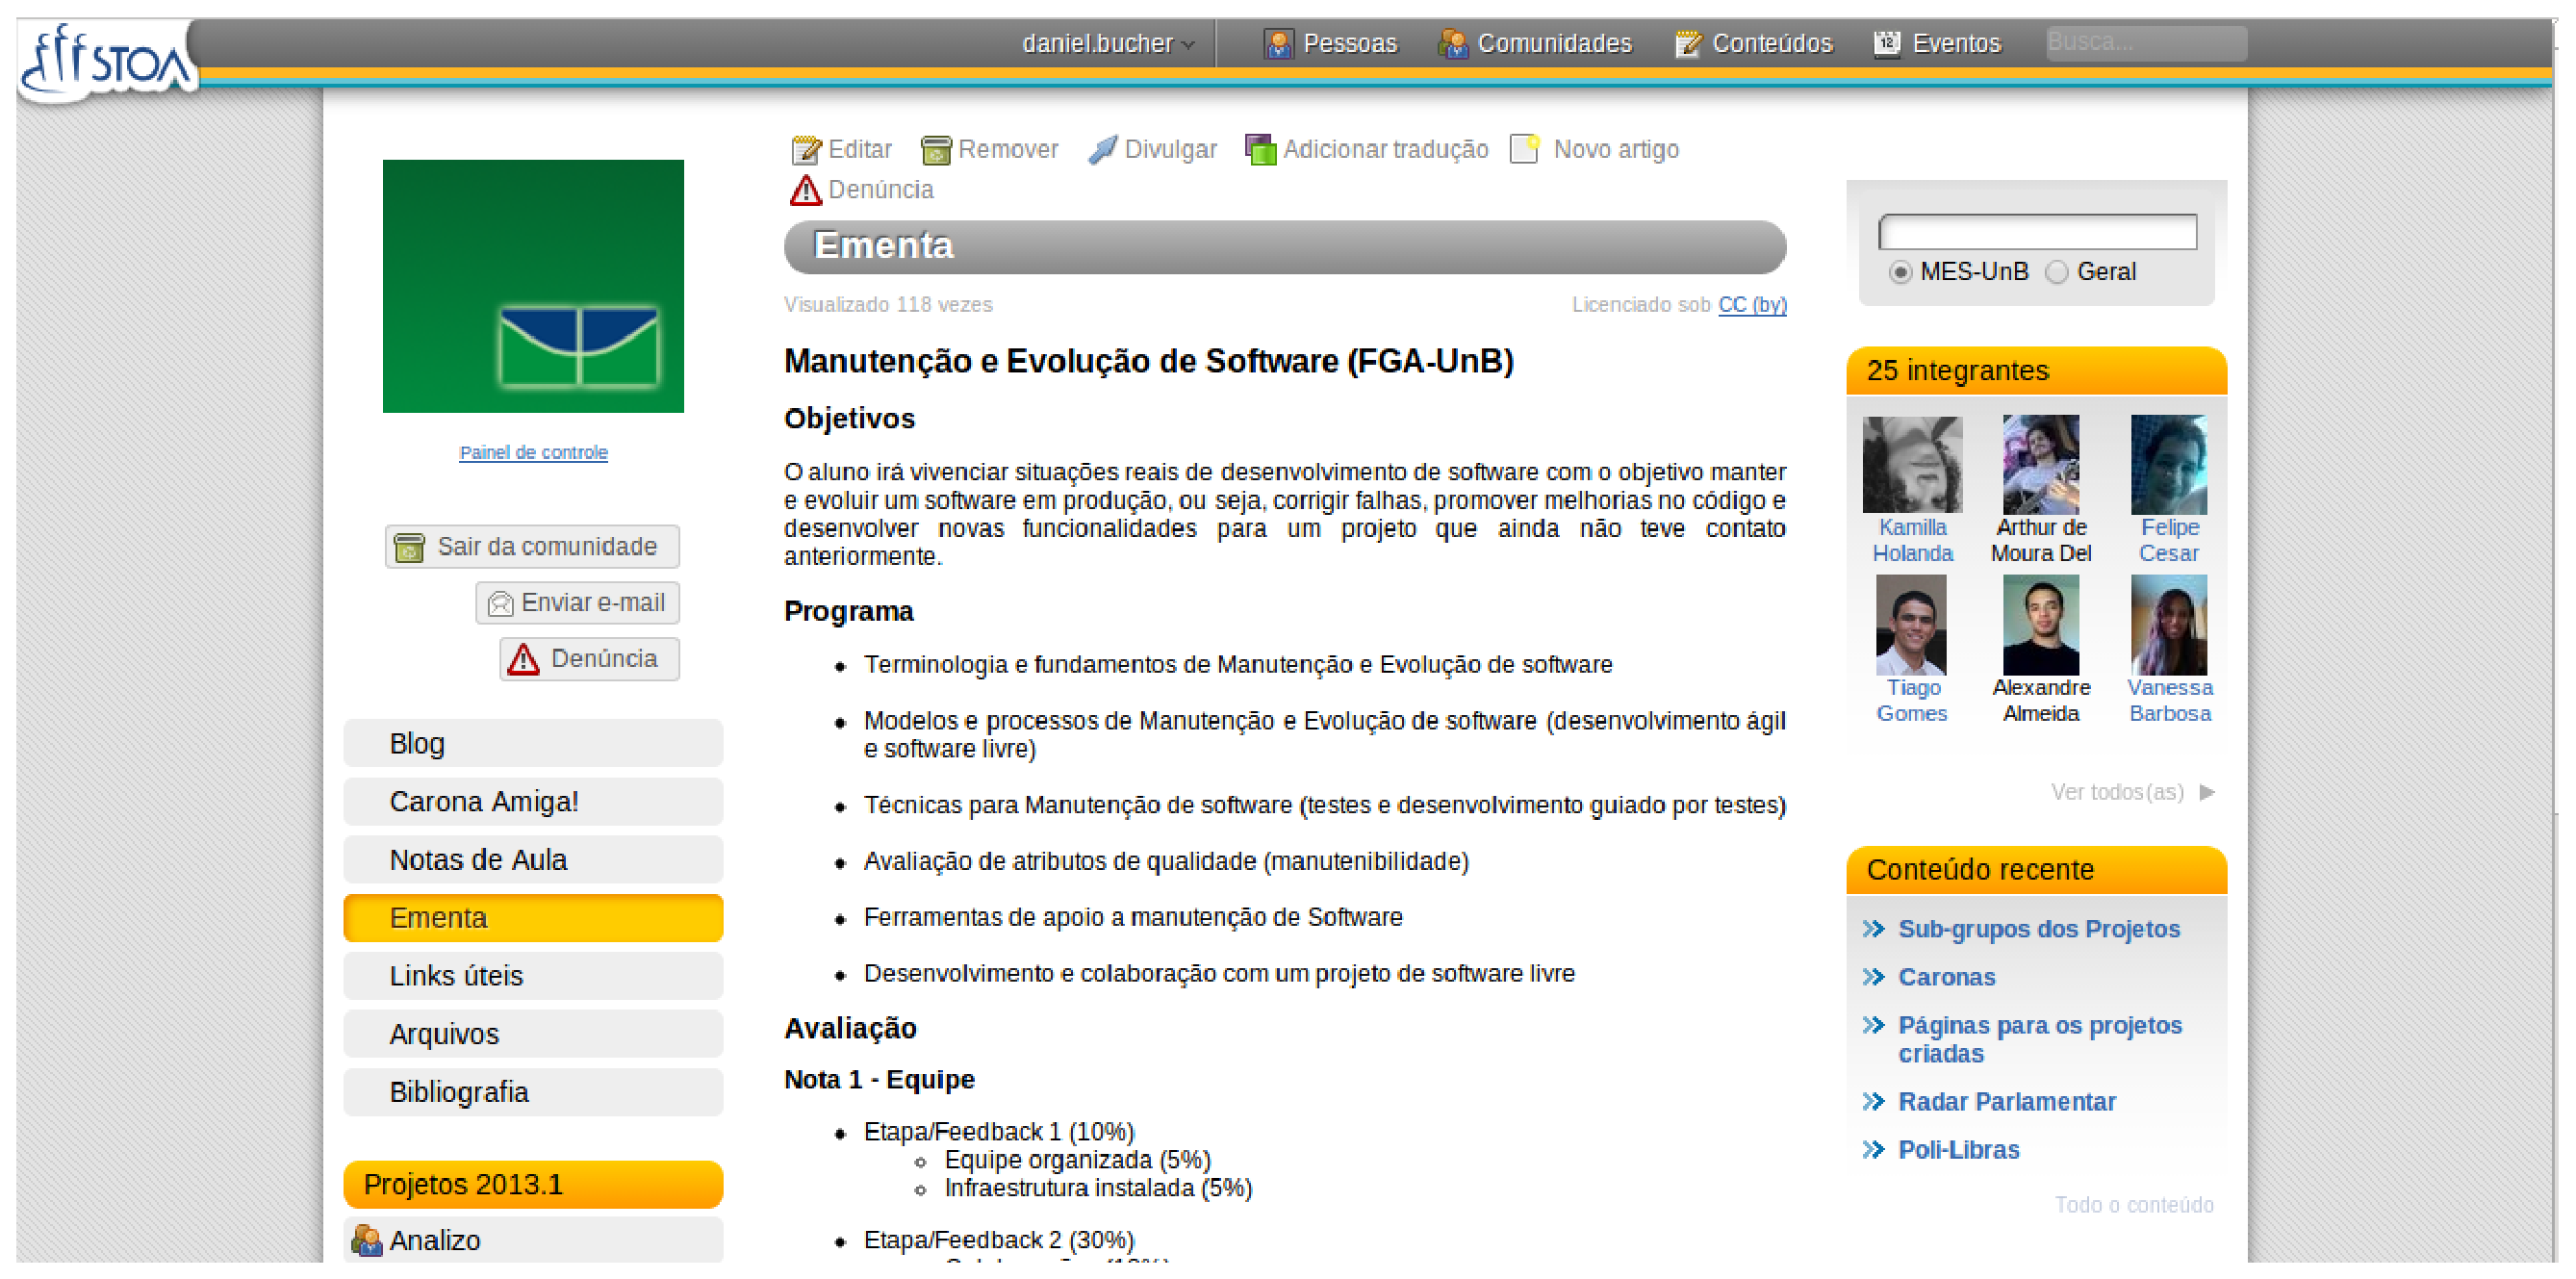
\includegraphics[keepaspectratio=true,scale=0.3]
	  {figuras/mes-unb.eps}
	\caption{Comunidade da disciplina de Manutenção e Evolução de Software}
	\label{mes-unb}
\end{figure}

A Figura \ref{analizo} apresenta o \textit{blog} do sub-grupo
criado para o projeto de manutenção na ferramenta Analizo~\footnote{Disponível
em \url{http://social.stoa.usp.br/analizo}}, uma ferramenta livre
para análise estática de código. O grupo optou por utilizar o \textit{blog}
para publicar o progresso do projeto no formato de \textit{release notes} e
retrospectivas dos ciclos de desenvolvimento.

\begin{figure}[h]
	\centering
	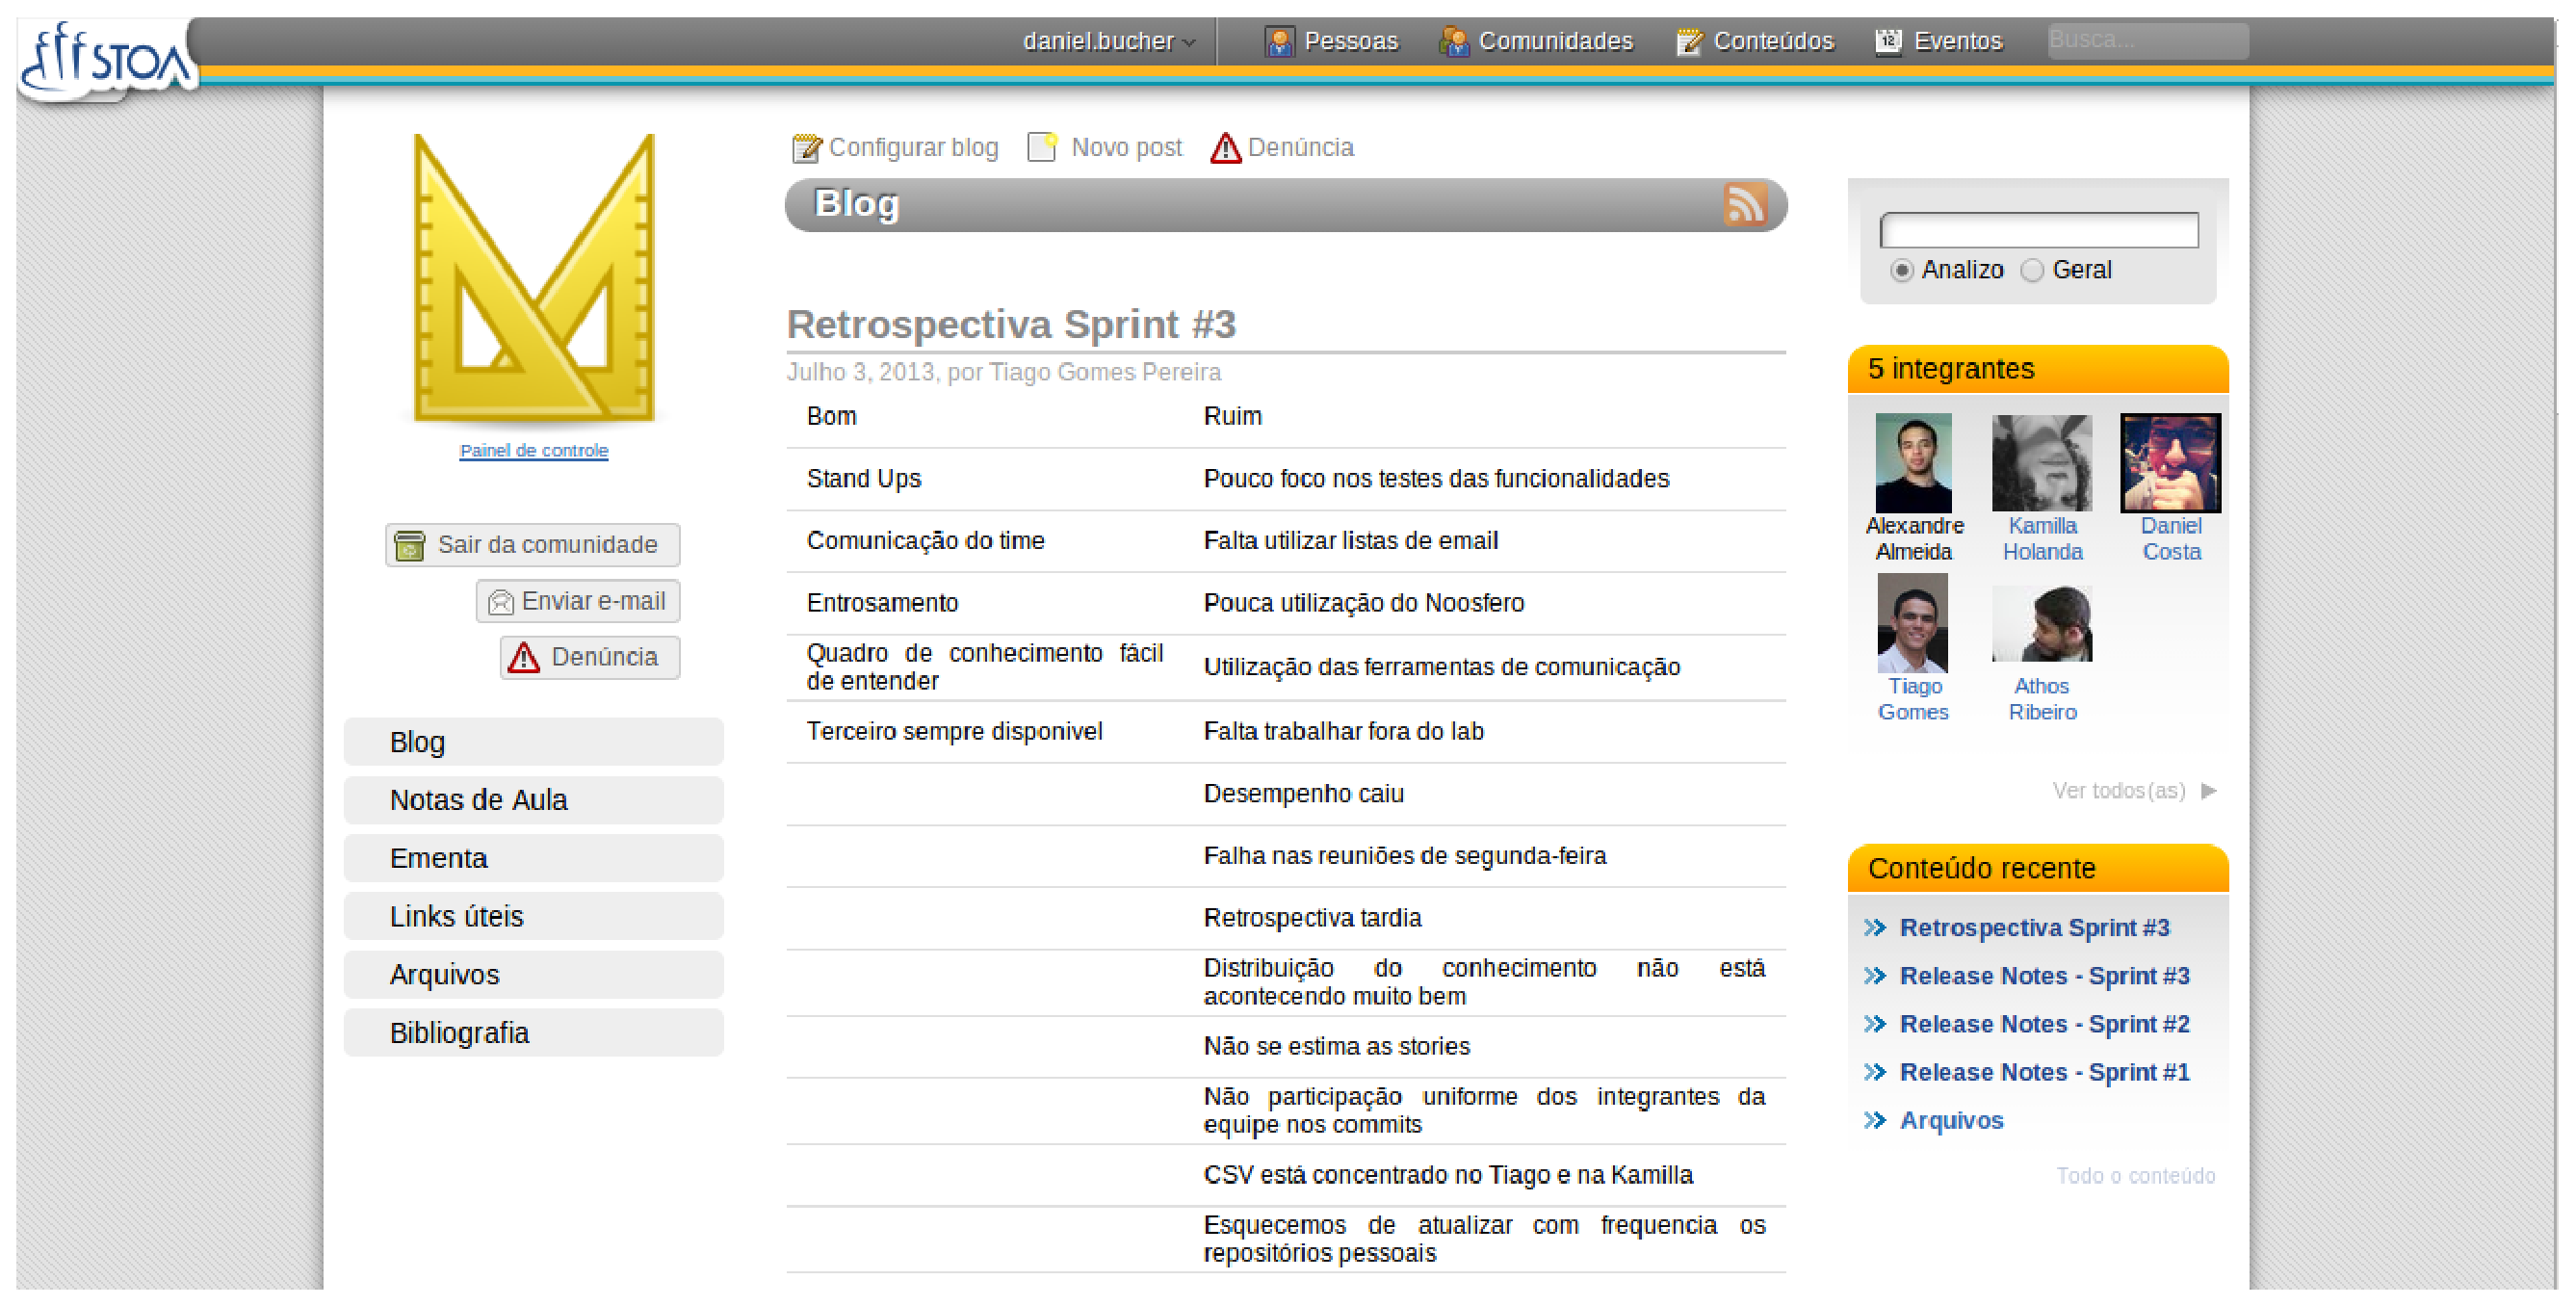
\includegraphics[keepaspectratio=true,scale=0.3]
	  {figuras/analizo.eps}
	\caption{Blog do sub-grupo do projeto Analizo da disciplina de MES }
	\label{analizo}
\end{figure}

